

\documentclass[10pt,onecolumn]{RequimentsGathering}

%
% All KJN's macros and goodies (some shameless borrowing from SPL)
\usepackage{KJN}
%\usepackage[hyphens]{url}

%
% PDF Info
%
\ifpdf
\pdfinfo{
/Title (SOFTWARE ENGINEERING PROJECT: STUDENTS MARKS/RECORDS MANAGEMENT SOFTWARE)
/Author (Khosa Masana (559990), Sanele Gcaba(459380), Tshegofatso Misapitso (600313), Londiwe Ngema (448871) )
/ModDate (D:200510121530)
/Subject (ELEN417/455 Paper Format, 2005)
/Keywords (ELEN417, ELEN455, paper, instructions, style guidelines, laboratory project)
}
\fi

%%%%%%%%%%%%%%%%%%%%%%%%%%%%%%%%%%%%%%%%%%%%%%%%%%%%%%%%%%%%%%%%%%%%%%%%%%%%%%%
\begin{document}

\begin{titlepage}

\newcommand{\HRule}{\rule{\linewidth}{0.5mm}} % Defines a new command for the horizontal lines, change thickness here

\center % Center everything on the page
{\small School$\;$of$\;$Electrical$\;$and$\;$Information$\;$Engineering,$\;$University of$\;$the$\;$Witwatersrand,$\;$Private$\;$Bag$\;$3,$\;$2050,$\;$Johannesburg,$\;$South$\;$Africa}\\[1.5cm] % Name of your university/college

\textsc{ELEN 4009 - Software Engineering}\\[0.5cm] % Major heading such as course name

\HRule \\[0.4cm]
{ \large \bfseries Student Marks/Records Management Software - Requirements Gathering}\\[0.4cm] % Title of your document
\HRule \\[1.5cm]

 \large

\textbf{Project Team :}
Khosa$\;$Masana$\;$(559990),
Sanele$\;$Gcaba$\;$(459380),
Tshegofatso$\;$Misapitso$\;$(600313) and
Londiwe$\;$Ngema$\;$(448871)


{\large \today}\\[3cm] % Date, change the \today to a set date if you want to be precise

%\includegraphics{Logo}\\[1cm] % Include a department/university logo - this will require the graphicx package

\vfill % Fill the rest of the page with whitespace

\end{titlepage}

\pagestyle{plain}.
\pagenumbering{roman} 
\tableofcontents 

\newpage

\section*{Document Status Sheet}

\begin{center}
    \begin{tabular}{ | p{5cm} | p{7cm} |}
\hline
\textbf{Document Title}& Software Requirements\\ \hline
\textbf{Authors} & M.$\;$Khosa, S.$\;$Gcaba, T.$\;$Misapitso, L.$\;$Ngema \\ \hline
\textbf{Version} & 0.01 \\ \hline
\textbf{Document Status} & Draft  \\ \hline

    \end{tabular}
\end{center}


\begin{center}
    \begin{tabular}{ | p{2cm} | p{3cm} | p{5cm} | p{5cm} |}
    \hline
    \textbf{Version}& \textbf{Date}& \textbf{Author(s)} & \textbf{Summary} \\ \hline
    0.0.1 & 25-02-2016 & M.$\;$Khosa, S.$\;$Gcaba, T.$\;$Misapitso, L.$\;$Ngema& Document Creation. \\ \hline

    \end{tabular}
\end{center}

\newpage


%%%%%%%%%%%%%%%%%%%%%%%%%%%%%%%%%%%%%%%%%%%%%%%%%%%%%%%%%%%%%%%%%%%%%%%%%%%%%%%
%
\pagestyle{plain}.
\pagenumbering{arabic} 
\section{Introduction}
\subsection{Purpose}

The purpose of this document is to present a detailed description of the requirements for the student marks/record system. It will state the purpose and features of the system, the interfaces of the system, what the system will do, the limitations under which it must operate, define inputs and the expected reaction of the system (that is the outputs of the system). 
\subsection{Project Scope}
This software system will be a marks record system. It is a convenient way for students to have access to their marks in a safe and confidential way as opposed to accessing them on notice boards where everyone else can publicly see them. The primary function of the application is to allow students to log-in using their details and be able to access their course marks. The users will be able select the academic year which they require marks for and the specific courses, course code, mark and symbol will be displayed to them. The program should have domains i.e. staff members can be able to access and edit the database while students can only view their individual marks. The system would be accessed online via a Browser and a Smart-phone App.
\subsection{List of Definitions and abbreviations}

\subsubsection{Definitions}

\subsubsection{Abbreviations}
%%%%%%%%%%%%%%%%%%%%%%%%%%%%%%%%%%%%%%%%%%%%%%%%%%%%%%%%%%%%%%%%%%%%%%%%%%%%%%%
%
\section{Expanded Description of the project}

The software system will follow a Two-Tier Architecture due to its ease of use and maintainability as compared to a Three-Tier Architecture. However, the performance of a Two-Tier Architecture slows down with an increase in users \cite{ref3}, hence a Three-Tier Architecture will be implemented with an increase of the number of users. Figure 1 below shows the Two-Tier Architecture.   
\begin{center}
\begin{figure}[h]
\centering
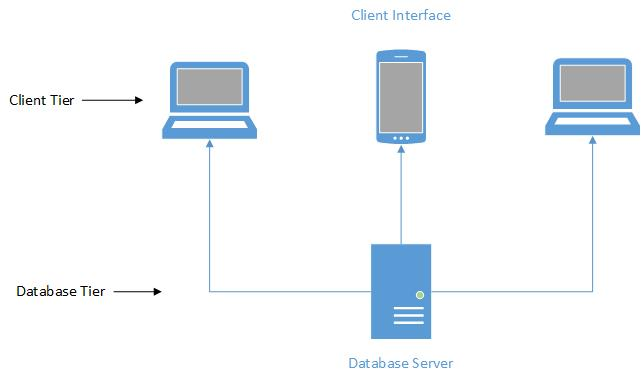
\includegraphics[width=10cm]{Two-Tier}
\caption{Two-Tier Software Architecture}
\end{figure}
\end{center}


"A Two-Tier Architecture is a software architecture where the interface runs on client and the data layer is stored on a server" \cite{ref4}.
\subsection{Front-End}

Khosa Masana (559990) and Londiwe Ngema (448871) are going to be responsible for the design, development and documentation of the front end (user interface).

Both the user interface of the browser and the smart-phone app are going to be designed using HTML5, CSS and JavaScript. The user interface will offer a platform whereby the users are going to interact with the server. The users (i.e students and staff) will be prompted for a student/staff number and a password to view or change the results. Only the staff members (lecturers) will be given the right to change the results, students can only view the results. Validation of credentials will be done in Javascript before they are submitted to the server.  

\subsubsection{\textbf{System Input and Output:}} 
 
With the student number, password and year entered as an input, the relevant information (results) of that particular student and the particular year will be searched from the server and displayed to the student. Results (Output) will be displayed in a form of a table with course name, course code, results and a symbol as columns. PHP will be used to link the back-end and front-end

\subsection{Back-End}
Sanele Gcaba (459380) and Tshegofatso Misapitso (600313)  are going to be responsible for the design, development and documentation of the back-end (Server and Database).

The back-end:
The proposed design of the back-end is to include a Linux Apache MySQL PHP(LAMP) install.

The Linux operating system is chosen for the server to run on because of its Stability, Security and Cost of operation \cite{ref1}.   
As a result centOS (minimal), a Linux operating system was chosen.
The Linux is Just the base of the project that will allow the server to run off. The server proposed is an Apache server. This server is chosen because it is easy to install and operate. Apache will provide a secure, efficient and extensible server that provides HTTP services.
The project requires that data is stored and later on read from. There is multiple datasets that need to be considered: for example multiple students that may be doing multiple courses and as a result a need for storing this data. MySQL was chosen because it is an open source database and large companies use it to save money and time powering their high volume websites \cite{ref2}.

PHP is  selected as the scripting language. This is chosen because of the simplicity of the language and in addition JavaScript can be used to do client side validation to avoid overloading the server with server side validation. Validation would be necessary for authentication. 
PHPMyadmin may be used in order to get a visual look of the database instead of having to type out queries in order to check that the data one expects to be in the database IS ACTUALLY IN THE DATA BASE. As a result PHPmyadmin could be used in testing of the script in terms of database manipulations.

Interacting: the client tries logging in:

\begin{itemize}
\item Client enters credentials, these credentials get validated ‘onsubmit’.
\item If the credentials are correct: a PHP script is used to determine if the user is a  student or staff member.
\item If the user is a student then the student will only have certain privileges such as reading from the database  only.
\item If the user is an administrator or a staff member then they may be allowed to have different privileges to edit the database: such as alter student results and add new student onto the database.
\end{itemize}

\vfill

%\nocite{*}
\bibliographystyle{witseie}
\bibliography{sample}

%{\tiny \vfill \hfill \today \hspace{5mm} witseie-paper-2003.\TeX}

\end{document}

" vim: ts=4
" vim: tw=78
" vim: autoindent
" vim: shiftwidth=4
